\documentclass[a4paper,11pt]{article}
\usepackage[top=1in, bottom=1in, left=0.5in, right=0.5in]{geometry} 
\usepackage{graphicx}
\usepackage{hyperref}
\usepackage{caption}
\usepackage{subcaption}
\usepackage{color}

\title{CS296 Project Report}

\author{
  Nehal Bhagat\\
  \texttt{Roll No.:110050008}\\
  \and
  Tanmay Randhavane\\
  \texttt{Roll No.:110050010}\\
  \and
  Ayush Kumar\\
  \texttt{Roll No.:110050038}\\
}

\begin{document}

\maketitle

\newpage


\tableofcontents
\newpage

\section{Original Rube-Goldberg Design}
{
\textbf{Initial Vs. Final Design}
\begin{figure}[h]
    \centering
    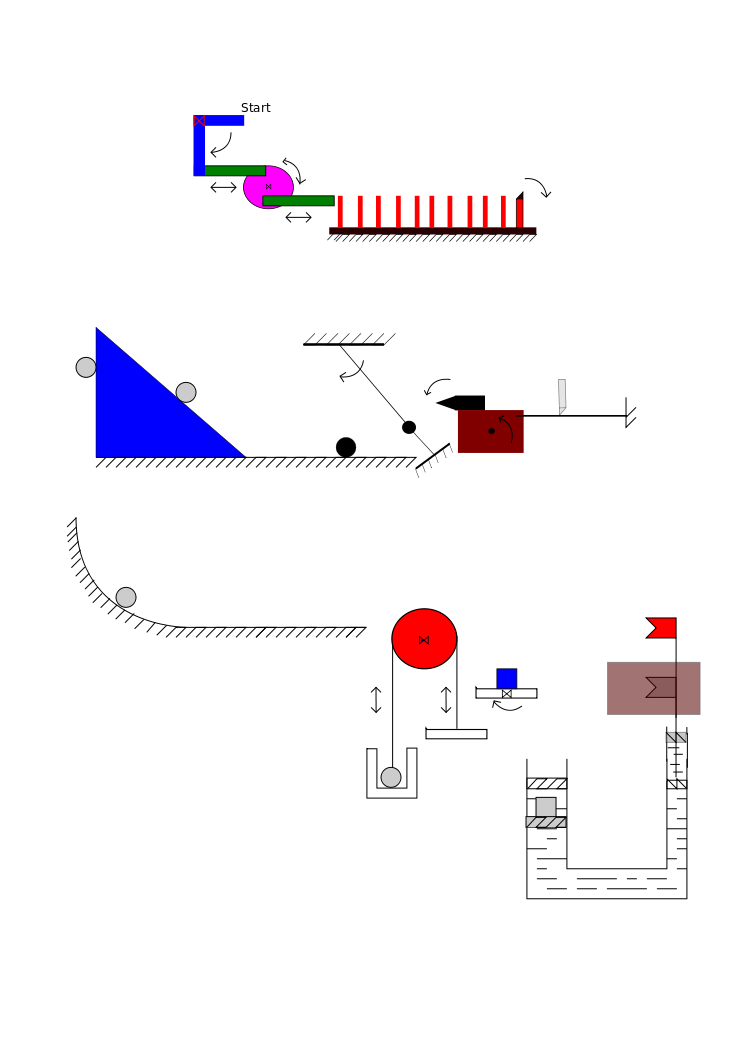
\includegraphics[scale=0.45]{images/rube-goldberg}
    \caption{Original Rubegoldberg Machine}
\end{figure}
  
\newpage
\begin{figure}[h]
    \centering
    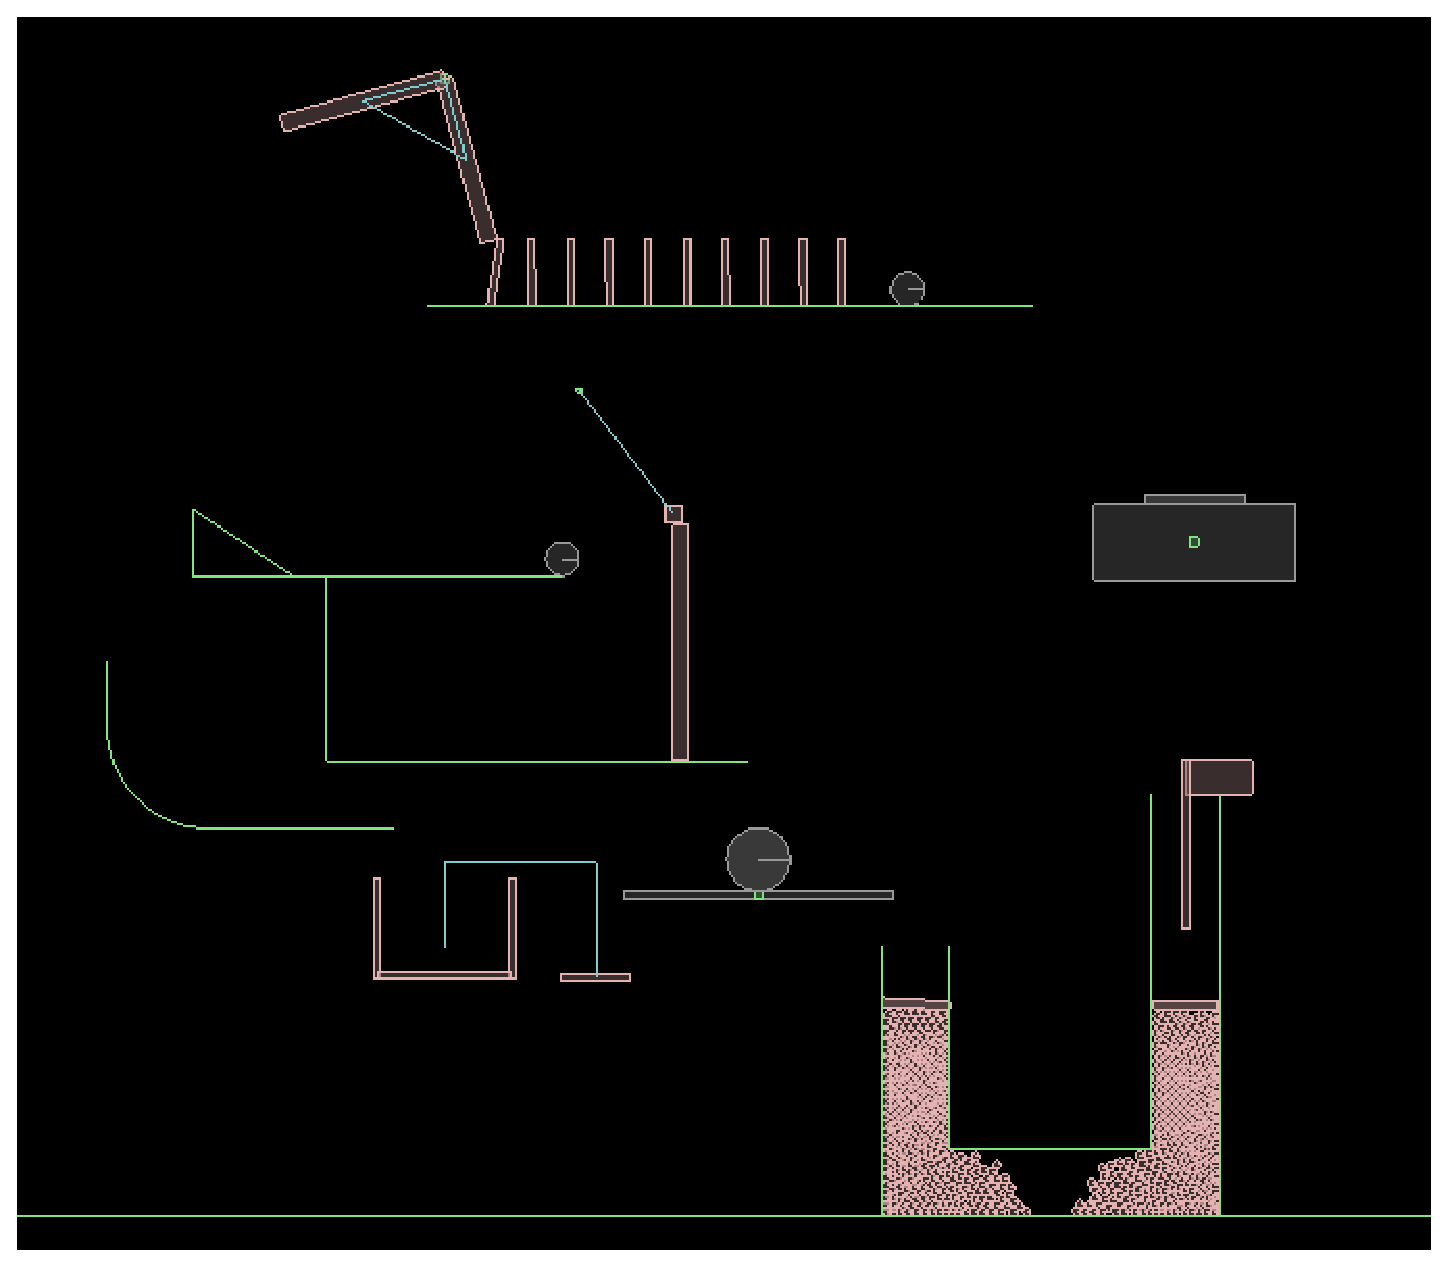
\includegraphics[scale=0.6]{images/final_rg}
    \caption{Final Rubegoldberg Machine}
\end{figure}
\newpage

\indent \indent Our original design of Rube-Goldberg design is shown in following figure. It works as follows. \\
\indent There is an L-shaped object hinged at the middle whose one end is connected to the bar. The other end of the bar is connected to the top of the axle. Similarly One other bar is connected at the bottom of the axle as shown in figure 1 \ref{fig:trigger}\\

\begin{figure}[h]
    \centering
    \label{fig:trigger}
    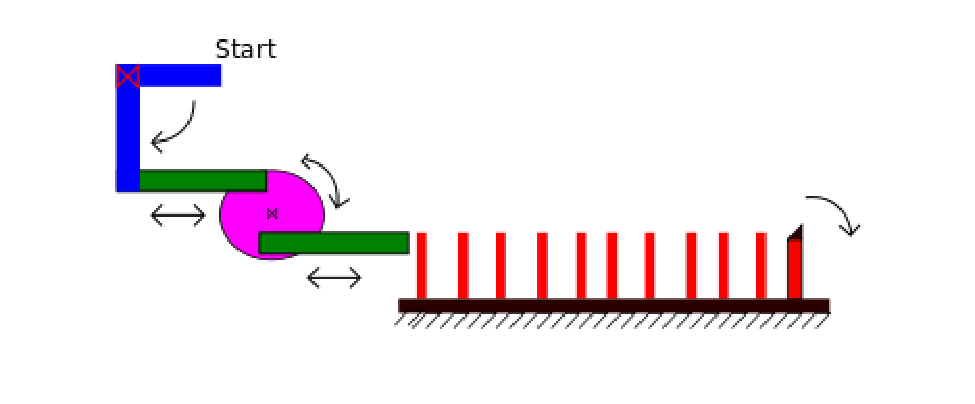
\includegraphics[scale=0.6]{images/trigger}
    \caption{Axle}
\end{figure}

\indent Initially the L-shaped object is positioned as shown in the figure 1, one of it's bar is in horizontal position and other in vertical. Hence it will start oscillating causing axle to oscillate in anti-clockwise direction first and then in clockwise direction. Thus bar connected at the bottom of the axle will move backward and then forward. Its forward motion will topple dominoes. \\

\indent There is another structure at the bottom of the last domino, as shown in the figure 2 \ref{fig:image1}.  It is a box hinged at it's center of mass. One of it's corner (right-up) is tied with a string which is connected to the wall. One another sharp edged pentagon is kept on it as shown in the figure. The pentagonal object provides anticlockwise torque (due to it's weight) and the string provides the clockwise torque to the box about it's center of mass, hence initially it is in equilibrium. 
\begin{figure}[h]
    \centering
    \label{fig:image1}
    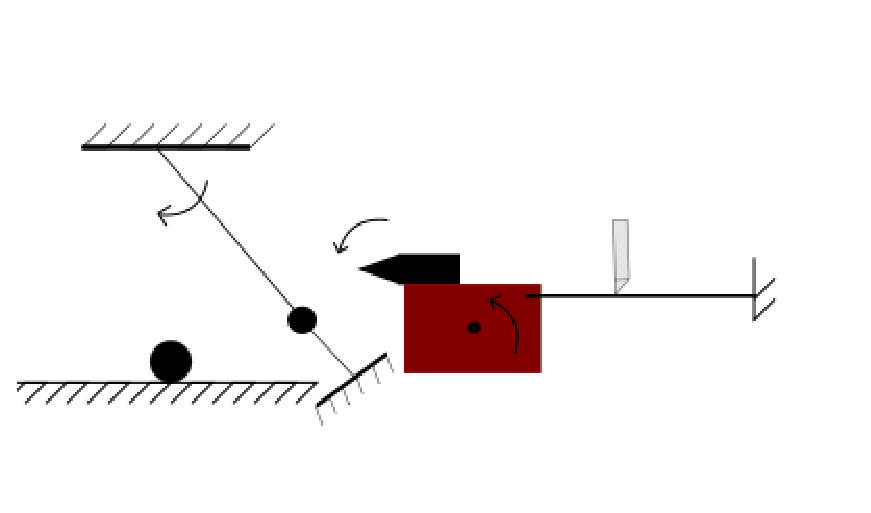
\includegraphics[scale=0.6]{images/image1}
    \caption{Structure below dominoes}
\end{figure}

\indent When the last domino is toppled, it falls on the string connected to the box and cuts it. Thus equilibrium of box is disturbed and it will rotate around the hinge in anticlockwise direction. As soon as the box rotates, the pentagonal object on it will fall on the another string which is connected to pendulum such that it's sharp edge cuts that string. When the string is cut the pendulum will start oscillations and hit the other ball. \\

\newpage
\indent Now this ball will move, climb the fixed wedge and then fall on the curved surface from the other side.
\begin{figure}[h]
    \centering
    \label{fig:image2}
    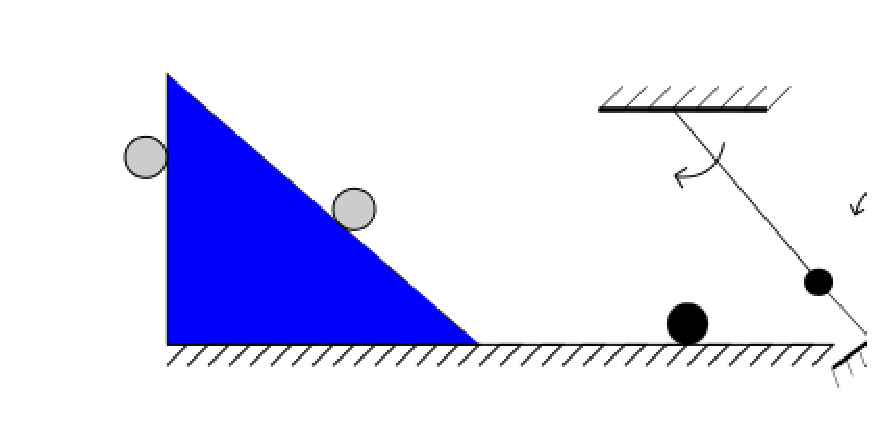
\includegraphics[scale=0.4]{images/image2}
    \caption{Ball climbing the fixed wedge}
\end{figure}


\indent After that it will move on the curved surface and fall into the container connected at one side of pulley.  
\indent Thus the horizontal bar, connected at the other side of pulley moves up and disturbs the equilibrium of hinged plank + box system as shown in figure 4. Thus box on this hinged plank will fall on the one of the end of the hydraulic lift. Thus according to principle of hydraulic lift, it's other side is pushed up. Finally the flag, symbol of success, is kept on the other end of hydraulic lift, is lifted up showing success. Refer figure 4 \ref{fig:image3}
\begin{figure}[h]
    \centering
    \label{fig:image3}
    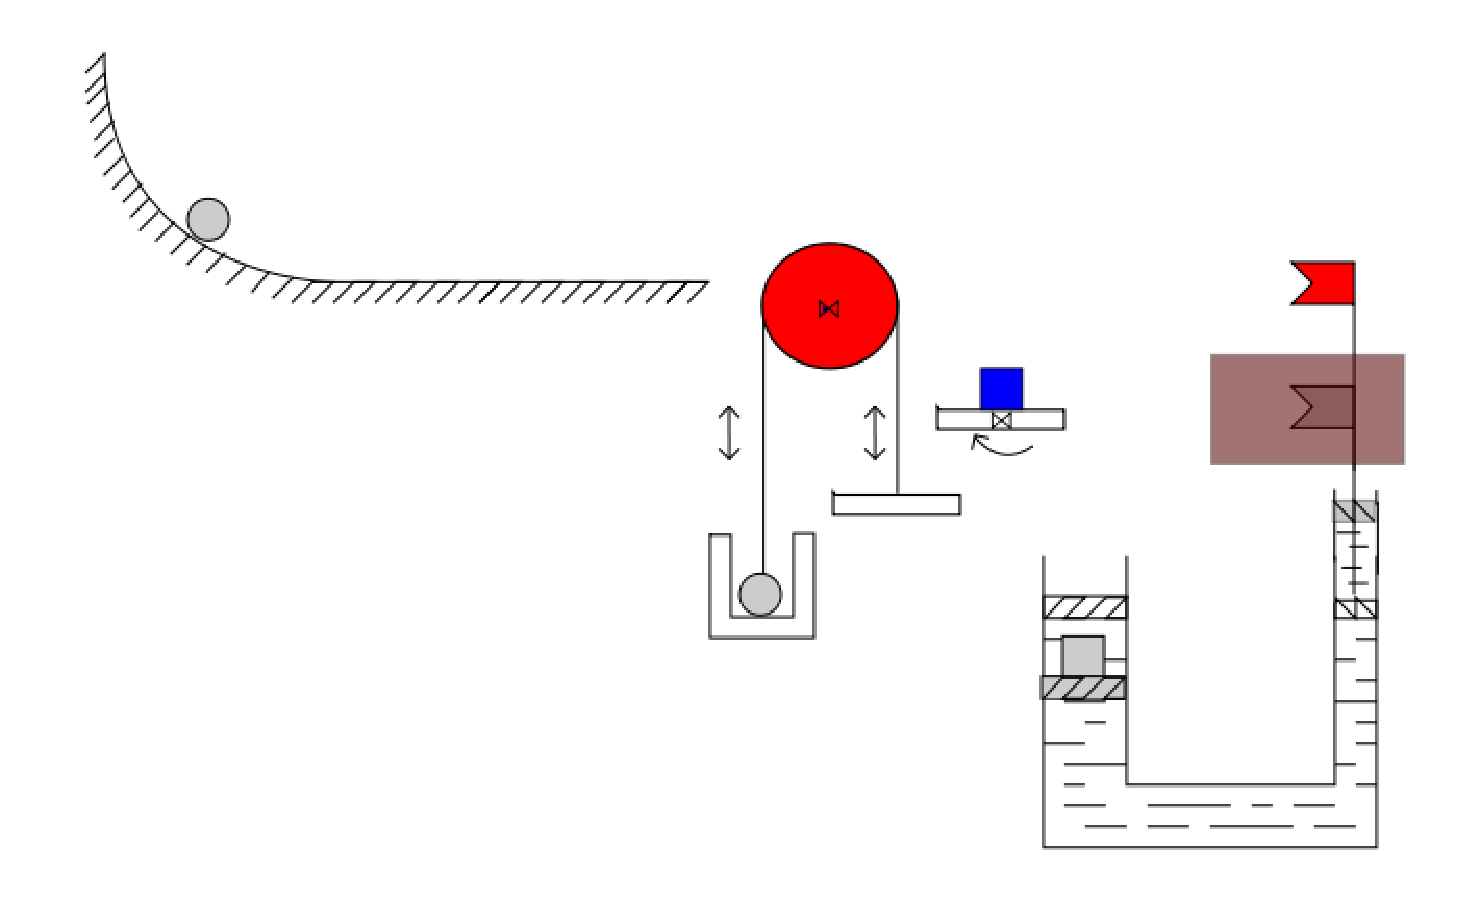
\includegraphics[scale=0.3]{images/image3}
    \caption{Motion of ball after it falls from the wedge}
\end{figure}

}

\newpage
\section{Final Rube-Goldberg Design}
{
\indent \indent The final design is very much similar to the original design. Followings are the changes done in original design. \\

1) Initial (L-shaped object, axle and bars connected at it's top and bottom) system (Figure 1 \ref{fig:trigger}) is replaced by the L-shaped object only. The L-shaped object is hinged at it's middle as shown in the figure. It will start oscillating, and it's motion will topple the dominoes. Refer figure \ref{fig:image4} \\
 In our original Implementation, we used axle to which two horizontal bars were connected at the bottom and at the top. Now there are two possibilities, either both of the bars are connected rigidly to axle or both are connected smoothly (axle and bar can freely rotate around the joint). \\
\indent If both of them were connected rigidly, then during oscillatory motion of L-shaped object, the upper bar will apply force in left direction on axle, but as axle is hinged at its center it cant move and thus axle will not rotate. \\
\indent If both of them were connected smoothly, then horizontal bar at the bottom of axle will rotate initially and try to become vertical. Thus it can't hit dominoes. Hence the replacement was done.

\begin{figure}[h]
    \centering
    \label{fig:image4}
    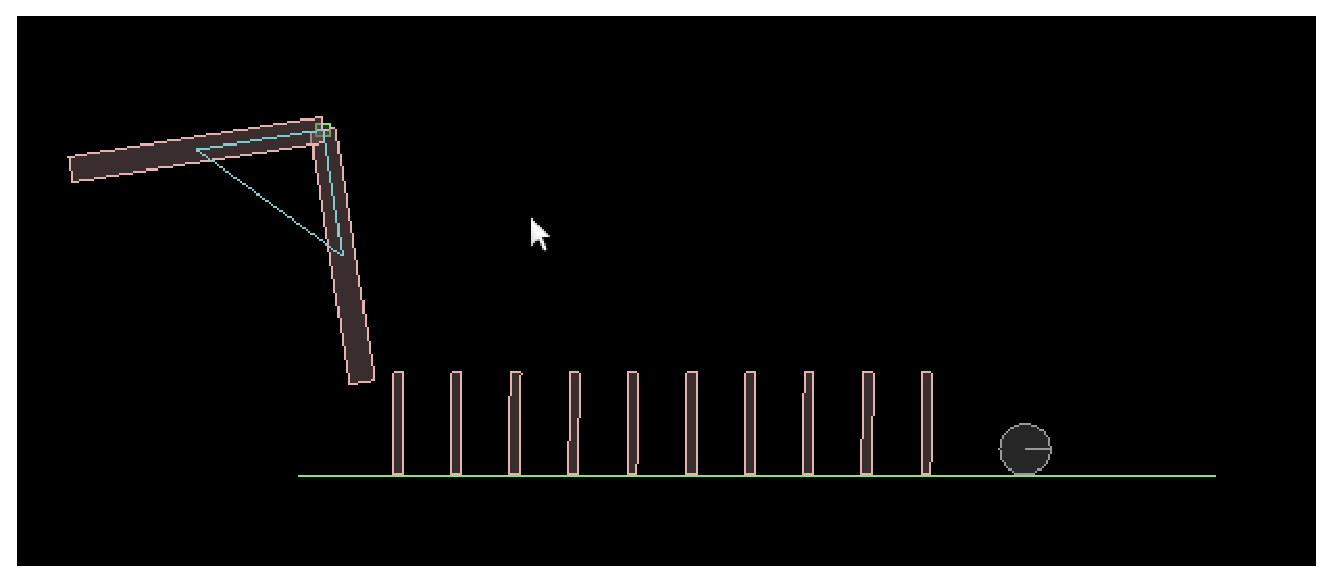
\includegraphics[scale=0.3]{images/image4}
    \caption{L-shaped object for triggering}
\end{figure}

2) In original design, the equilibrium of the box (shown in figure 2 \ref{fig:image1}) is disturbed by cutting the string. As string cutting is not possible in Box2d we did some changes. One bar is kept on this box at center. We made last domino to hit the ball kept in front of it. This ball will fall on the left side of this box and disturb it's equilibrium causing bar kept on it to perform projectile motion. 

\begin{figure}[ht!]
\centering
\begin{subfigure}{.5\textwidth}
  \centering
  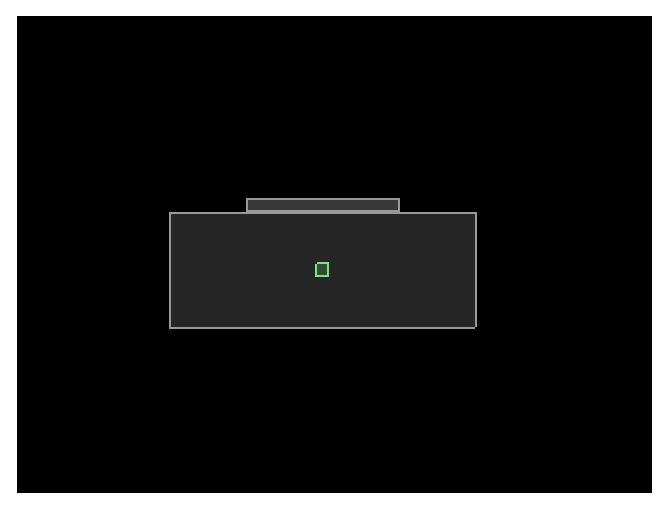
\includegraphics[width=.4\linewidth]{images/image5}
  \caption{At equilibrium}
  \label{fig:image5}
\end{subfigure}%
\begin{subfigure}{.5\textwidth}
  \centering
  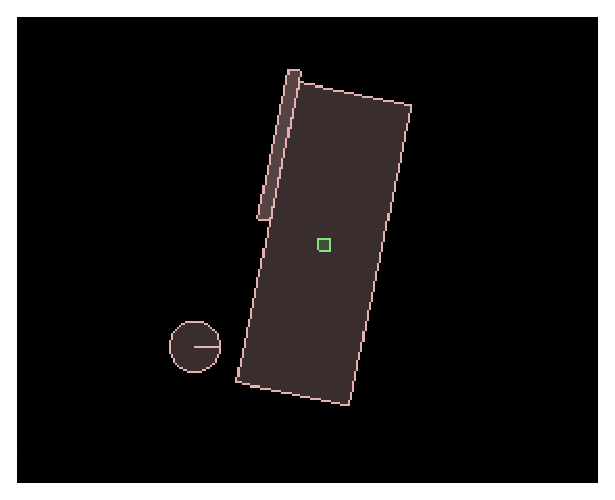
\includegraphics[width=.4\linewidth]{images/image6}
  \caption{equilibrium disturbed}
  \label{fig:image6}
\end{subfigure}
\end{figure}

3) In our original design, the pendulum was tied to the string (shown in figure 2 \ref{fig:image1}), and when string was cut it performed oscillations. As string cutting is not possible in box2D, we placed pendulum bob on the vertical support, and made it oscillate when this vertical support is disturbed (as shown in figure below). Here we disturbed it's vertical support by colliding it with the bar performing projectile motion as mentioned in 2nd point.\\

\begin{figure}[h]
\centering
\begin{subfigure}{.5\textwidth}
  \centering
  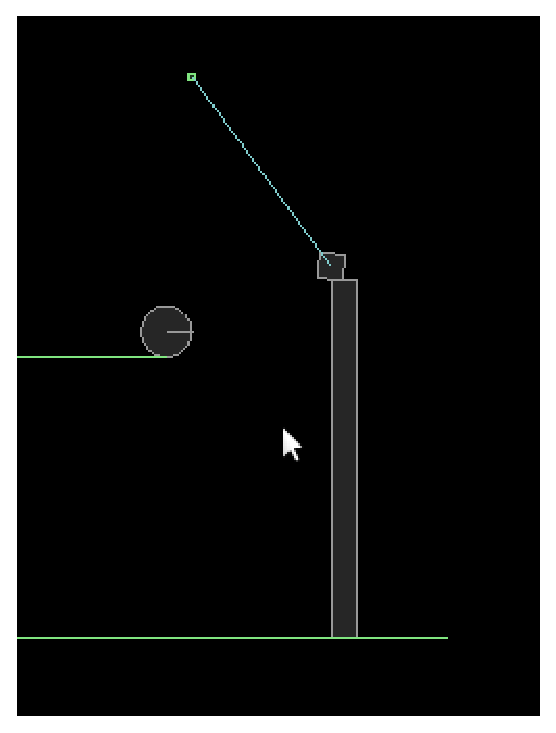
\includegraphics[width=.4\linewidth]{images/image7}
  \caption{At equilibrium}
  \label{fig:image7}
\end{subfigure}%
\begin{subfigure}{.5\textwidth}
  \centering
  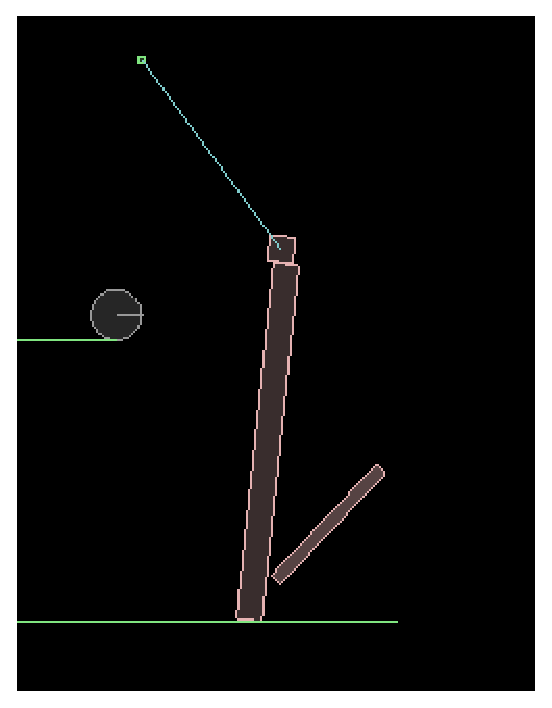
\includegraphics[width=.4\linewidth]{images/image8}
  \caption{equilibrium disturbed}
  \label{fig:image8}
\end{subfigure}
\end{figure}

\newpage
4) Water in hydraulic lift is implemented using large number of balls. As only rigid bodies can be implemented in box2D , water can't be implemented. \\

\begin{figure}[h]
    \centering
    \label{fig:image9}
    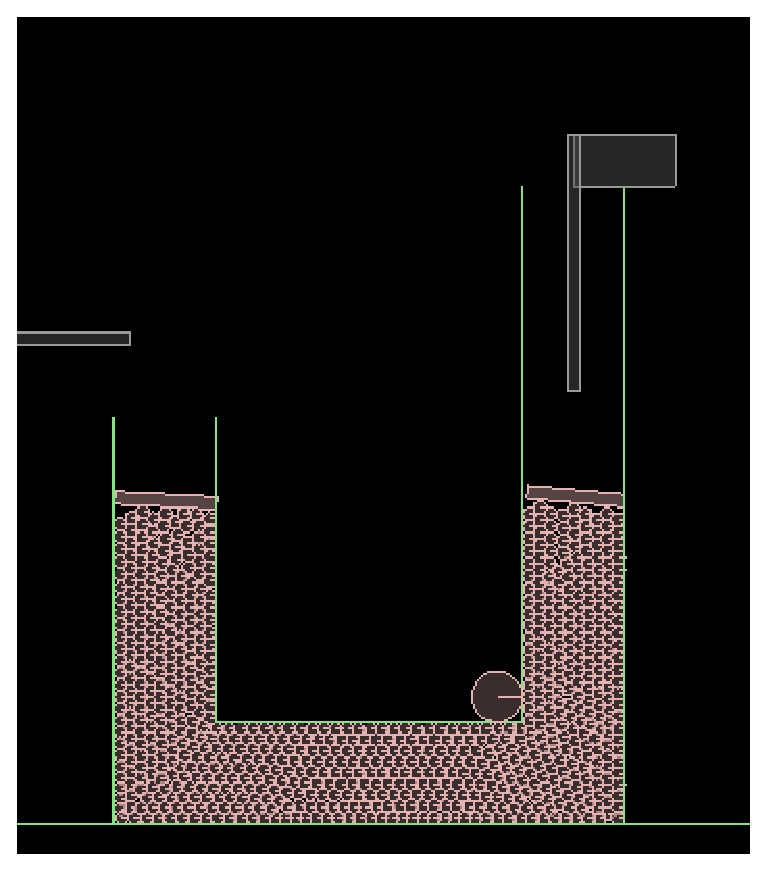
\includegraphics[scale=0.3]{images/image9}
    \caption{Hydraulic Lift}
\end{figure}

}

\newpage
\section{Interesting Things}
{
\indent \indent The most interesting part of our Rube-Goldberg machine is hydraulic lift. As we can only implement rigid bodies in Box2D, implementing water was a challenging task. We implemented it using large number of small balls. 
The flow of water when it tries to attain equillibrium is really awesome!\\

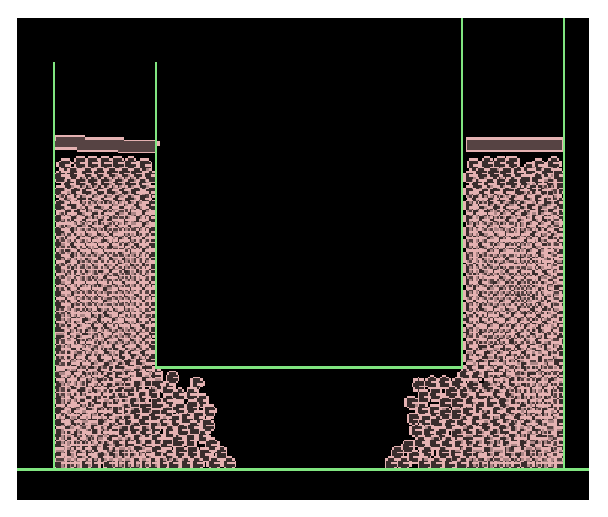
\includegraphics[scale = 0.4]{images/image10} \hspace{0.5in} 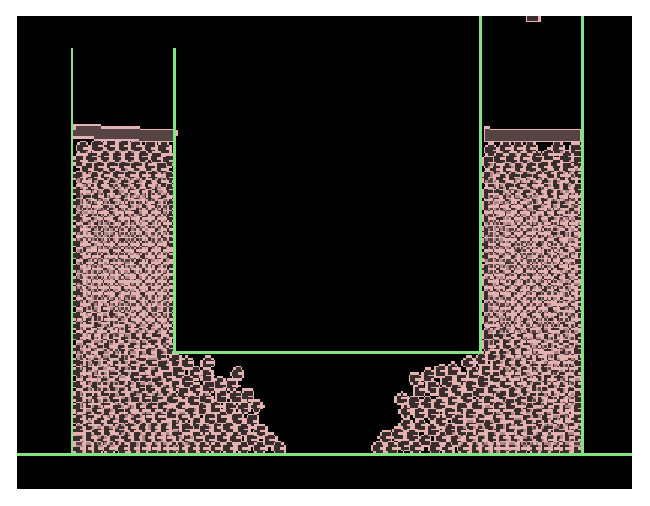
\includegraphics[scale = 0.4]{images/image11} \hspace{0.5in} 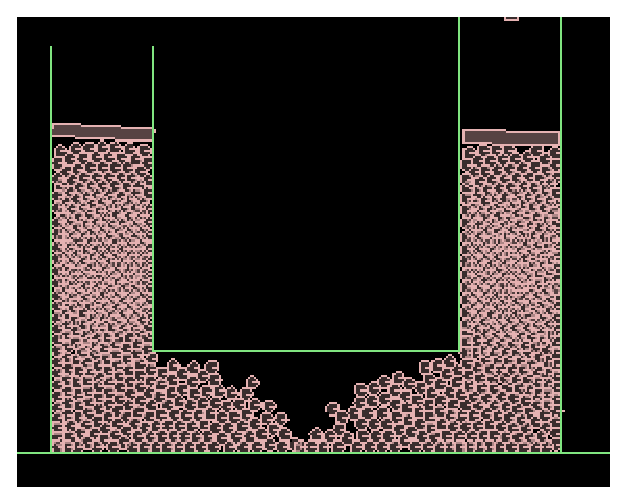
\includegraphics[scale = 0.4]{images/image12}
\\ \\
\indent And at the end, a flag is hoisted. We took this idea from the mario game. Whenever mario completes any level, a flag gets hoisted. It is a symbol of victory for him, as he successfully overcomes all the obstacles in his path and reaches destination. Thus flag in our rube-goldberg machine is a symbol of success
}

\newpage
\section{Profiling}
{
\subsection{Information from profiling data}
{

\indent \indent 1)Number of functions calls is less in release part as compared to that of debug part. In both the parts, the function b2Vec2::b2Vec2(float, float) is called for the maximum number of times. It is called 140000000 times in the release part whereas it is called 150000000 times in the debug part. Though these numbers though these numbers do not differ drastically, the time taken by this function in release part is 0.14 seconds whereas it is 0.23 seconds in debug form. This means, optimization worked in the release part and reduced the number of function calls may be replacing the function calls by actual function code. \\

2)Number of functions calls for constructors are drastically lesser in the release part as compared to debug part. This indicates that optimization flags work on constructors. \\

3)In both mode, the function b2World$::$ SolveTOI(b2TimeStep const) takes maximum time. In this function, time of impact is solved iteratively. In our design, we implemented water in hydraulic lift using large number of small particles (balls) which keep colliding once disturbed for long time, hence we can reduce friction coefficient and density of those particle to zero and one respectively. It will make calculation easy and take less time.

4) Even after optimization, the function SolveVelocityConstraints() takes most time. We can do the following optimization in the code for the function in Box2d library$:$ \\ \\
  \fbox{%
  \begin{minipage}{7.2 in}
  \indent In the function, SolveVelocityConstraints() of the Box2d library from the Dynamic/Contacts/b2ContactSolver.cpp file, there are many situations where a variable is defined which is used only once later in that loop. We could directly use the value instead of declaring the variable, \\
For example, in line 321,\\
  b2Vec2 dv = vB + b2Cross(wB, vcp-$>$ rB) - vA - b2Cross(wA, vcp-$>$rA);\\ \\
  a variable dv is defined which is used only once in line 324,\\
  float32 vt = b2Dot(dv, tangent) - vc-$> $tangentSpeed;\\ \\
  instead we could directly write \\
  float32 vt = b2Dot(vB + b2Cross(wB, vcp-$> $rB) - vA - b2Cross(wA, vcp-$>$rA), tangent) - vc-$>$ tangentSpeed; \\
  and remove the definition of dv altogether. Same optimization can be done in line number 349 too. Since this    function solveVelocityConstraints() is the function that takes most of the time, optimizations in it can be useful.
  \end{minipage}} 

}

\subsection{Analysis of call graph}
{

1) The call graph shows how much time was spent in each function and it's children.

\begin{figure}[h]
    \centering
    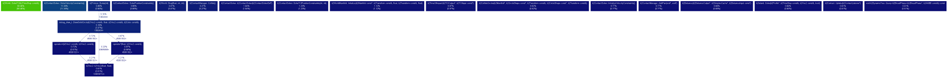
\includegraphics[width=17cm]{images/release}
    \caption{Call Graph for the release part}
\end{figure}

\begin{figure}[h]
    \centering
    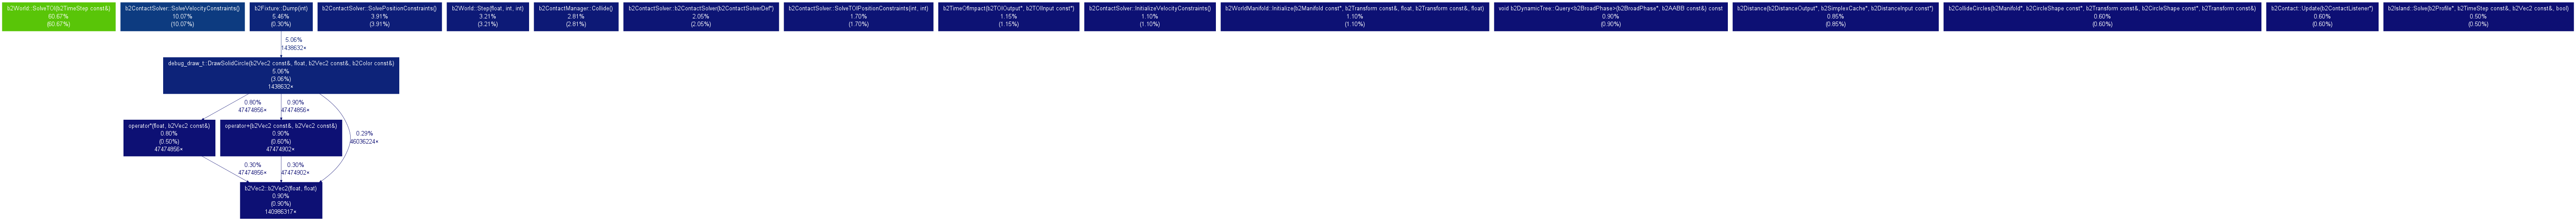
\includegraphics[width=17cm]{images/debug}
    \caption{Call Graph for the debug part}
\end{figure}


2)Call graphs obtained in both the parts, shows that the function b2Fixture$::$Dump(int) calls it's other functions namely b2Vec2$::$b2Vec2(float, float), operator+(b2Vec2 const\&, b2Vec2 const\&), operator*(float,b2Vec2 const\&) several number of times.

\begin{figure}[h]
    \centering
    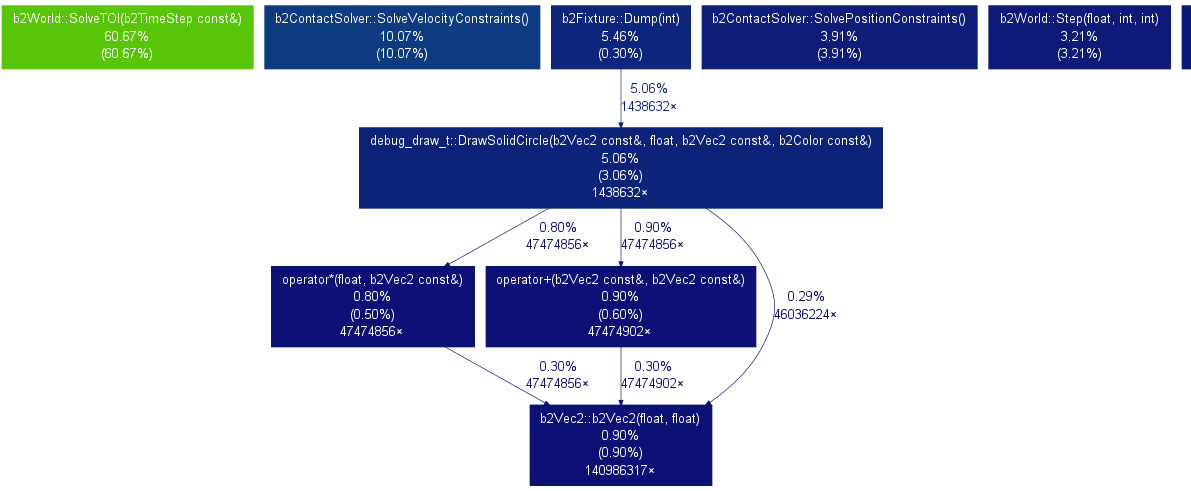
\includegraphics[scale=0.4]{images/debug_part}
    \caption{Part of Call Graph showing calls to children function}
\end{figure}


}

}

\newpage
\section{Analysis of Graphs}
{
\subsection{Loop time averaged over all reruns for various iteration values}
{
\indent \indent \textbf{Observation}$:$ Loop time averaged over all reruns (the points with the blue dots) increases linearly.\\
\indent \textbf{Explanation}$:$ The step() function of Box2D world detects that if an event is occurred or not, if yes, then corresponding callback is given. An increase in the iteration value means addition of time taken for an extra
 step function with a callback causing a significant increase in the loop time. Hence, we can see the significant
 increasing trend of loop times.
 
 \begin{figure}[h]
    \centering
    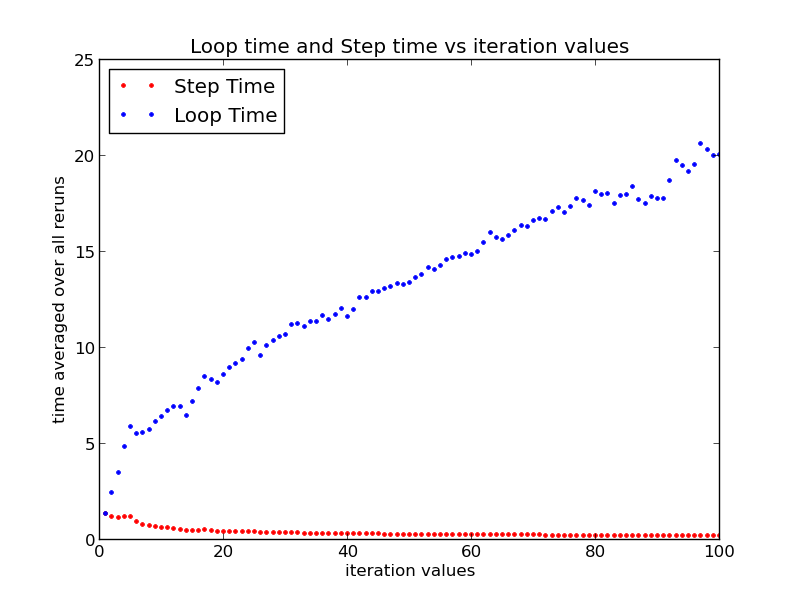
\includegraphics[scale = 0.5]{images/plot1}
\end{figure}
}


\subsection{Errors in the step time averaged over all reruns for various iteration values.}
{
\indent \indent \textbf{Observation}$:$ The length of y-error bars for lower iteration values is more as compared to the length of
 y-error bars for higher iteration values.\\
 
\begin{figure}[h]
    \centering
    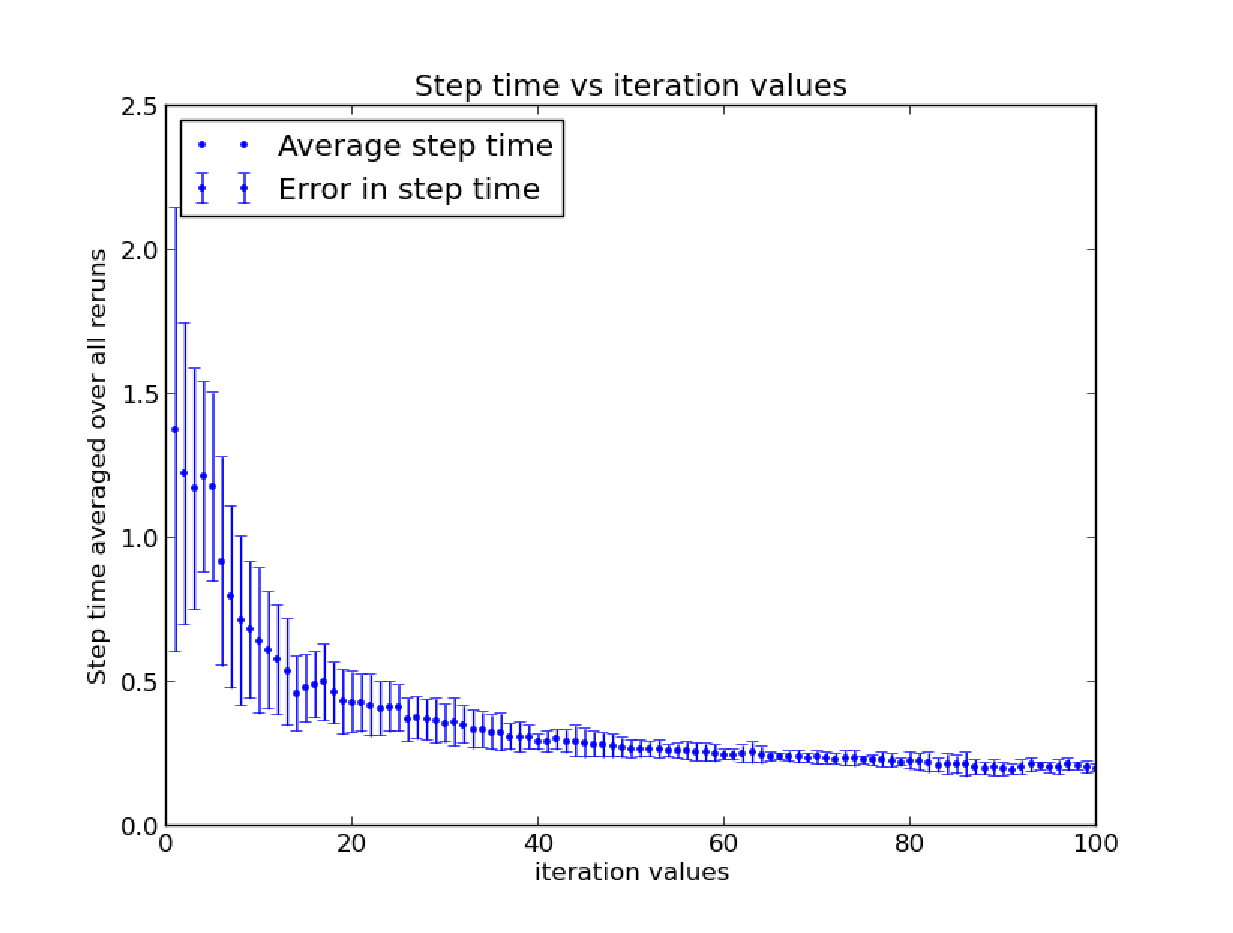
\includegraphics[scale = 0.5]{images/plot5}
\end{figure}



\indent \textbf{Explanation}$:$When iteration value is lower, the average step time is calculated for less number of steps
 which is then averaged over all reruns(100 reruns). Thus, less amount of data is available for averaging the
 values when iteration value is lower. Due to less data, the averages for lower iteration values are less accurate
 giving larger errors. Hence, the larger y-error bars for low iteration values.
}

\subsection{Values of times before and after adding load}
{
\indent \indent \textbf{Observation}$:$ Values of loop time for all iteration values and rerun values increase significantly when system is heavily loaded.\\

\indent \textbf{Explanation}$:$ If the system is heavily loaded, the function gets less share of CPU resources thus increasing the time of processing.\\

\begin{figure}[h]
\centering
\begin{subfigure}{.5\textwidth}
  \centering
  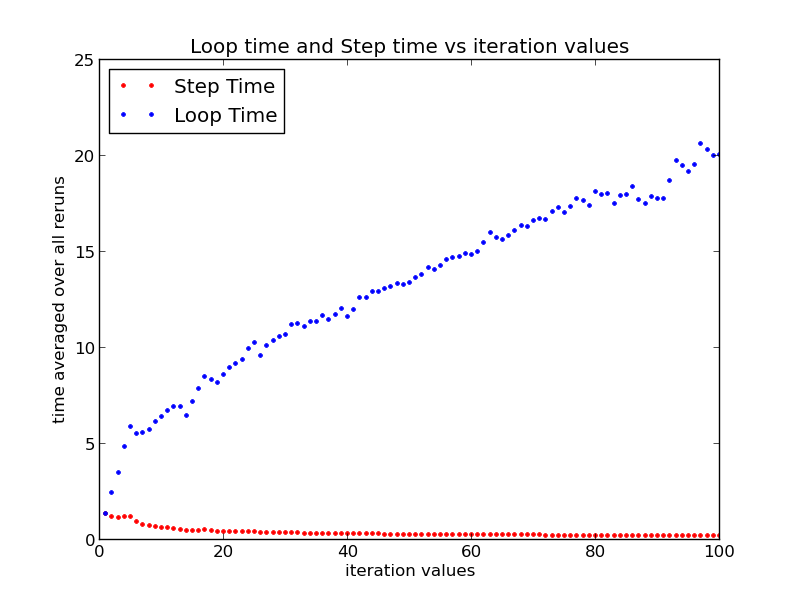
\includegraphics[width=1.0\linewidth]{images/plot1}
  \caption{Before load}
\end{subfigure}%
\begin{subfigure}{.5\textwidth}
  \centering
  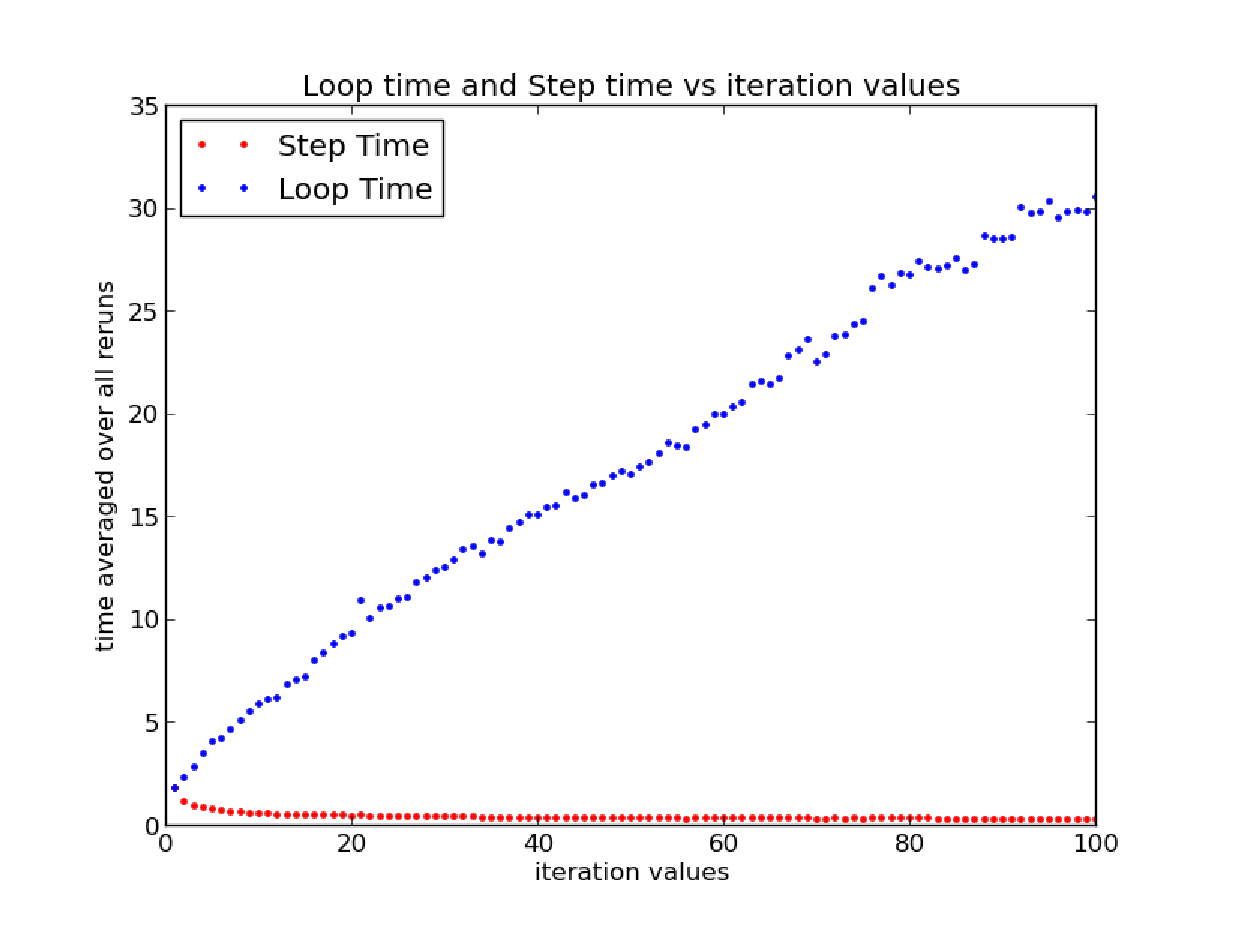
\includegraphics[width=1.0\linewidth]{images/plot2}
  \caption{After load}
\end{subfigure}
\end{figure}

\indent When system is without load slope of graph is approximately 0.21 ms/iteration, which means each iteration takes approximately approximately .21 ms. But in case of heavily load it is 0.30 ms which meas each extra iteration takes approximately 0.30 ms.

\begin{figure}[h]
\centering
\begin{subfigure}{.5\textwidth}
  \centering
  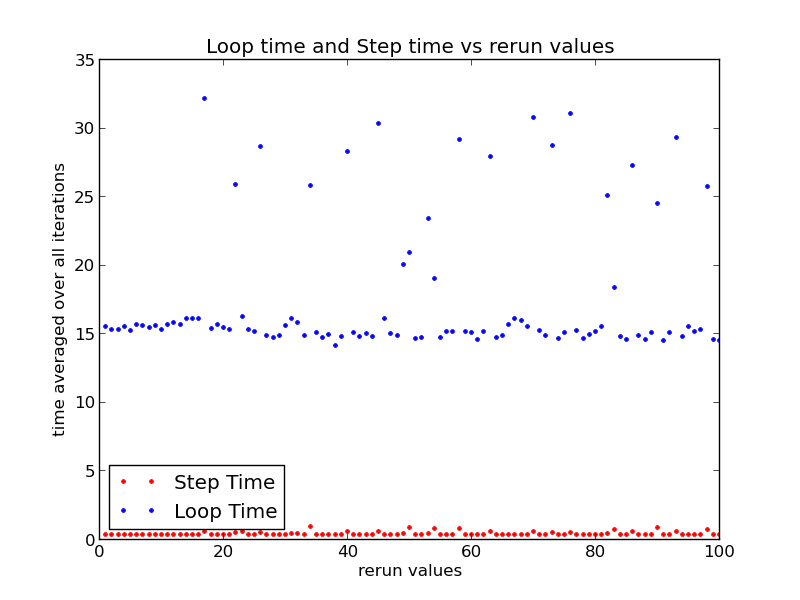
\includegraphics[width=1.0\linewidth]{images/plot3}
  \caption{Before load}
\end{subfigure}%
\begin{subfigure}{.5\textwidth}
  \centering
  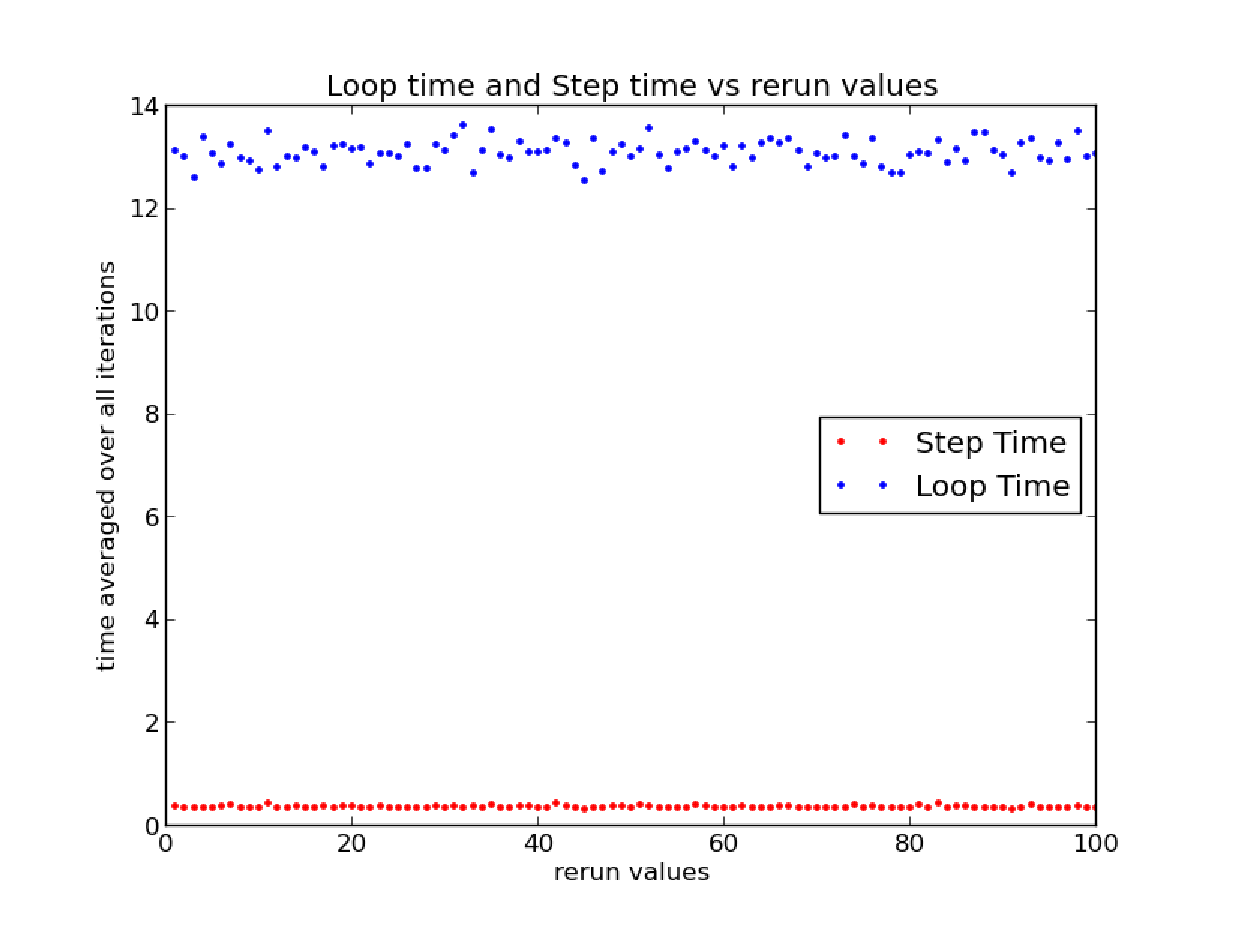
\includegraphics[width=1.0\linewidth]{images/plot4}
  \caption{After load}
\end{subfigure}
\end{figure}

\indent When system is less loaded, loop time averaged over all reruns is around 13ms and it is around 15 ms in case of heavy load with some variation. 
}



}


\newpage
\section{Bibliography}

\begin{thebibliography}{9}


\bibitem{k} Box2D Forums \url{http://box2d.org/forum/}
\bibitem{l} Stack Overflow \url{http://stackoverflow.com/}
\bibitem{m} github:help \url {https://help.github.com/}
\bibitem{n} Git - Getting a Git Repository \url {http://git-scm.com/book/en/Git-Basics-Getting-a-Git-Repository}
\bibitem{o} Python Call Graph \url {http://pycallgraph.slowchop.com/}
\bibitem{p} place multiple images on one line in latex or even create a matrix of images \url{http://desk.stinkpot.org:8080/tricks/index.php/2006/05/place-multiple-images-on-one-line-in-latex-or-even-create-a-matrix-of-images/}

\end{thebibliography}

\end{document}
